\section{Application of Agent-Based Model}

To simulate our agent-based model in real-world scenarios, we must choose three distinct plots of land from a temperate, arid, and tropical region with relatively low human interference. So, we randomly selected three "open" regions in the United States. The regions selected for the temperate, arid, and tropical regions are Clay, New York; Phoenix, Arizona; and Florida Keys, Florida, respectively. 

\subsection{Climate Calibration}

To calibrate our model to each selected region, we define several of our \textit{hyperparameters} from the previous section, which capture the difference in climate, consumers, and soil nutrition levels. We use the term hyperparameters to designate global values that are not directly passed into our model but still change the output of the model. 

\begin{itemize}
    \item Temperature — The local temperature (\(^\circ\)F) over 2022.
    \item Light Levels — The local average hours of sunshine over 2022.
    \item Potassium and Nitrogen Levels — Local potassium and nitrogen levels (ppm) in the local soil. (Note that since Potassium levels are closely correlated with soil moisture, we did not choose to calibrate our model with rainfall, as potassium was indicative enough).    
\end{itemize}

See Appendix 1 for more details on the implementation of our agent-based simulation. 

\subsection{Regional Results}

\subsubsection{Temperate Region: Clay, NY}
We obtained data detailing the local temperature, light level, soil composition, and wind data of Clay, NY to calibrate our model's \textit{regional hyperparameters} \cite{aladin_wolcott_nodate, us_department_of_commerce_nowdata_nodate}. Our results for this region are summarized in Figure~\ref{fig:temperatespread} where \(t\) represents time and \(n\) represents the number of dandelions. Additionally, the graphs are scaled to the dimensions of the open plot of land we began with (100 meters by 100 meters). Recall that our first dandelion started at coordinate \((0,0)\).

\begin{figure}[h!]
\centering
    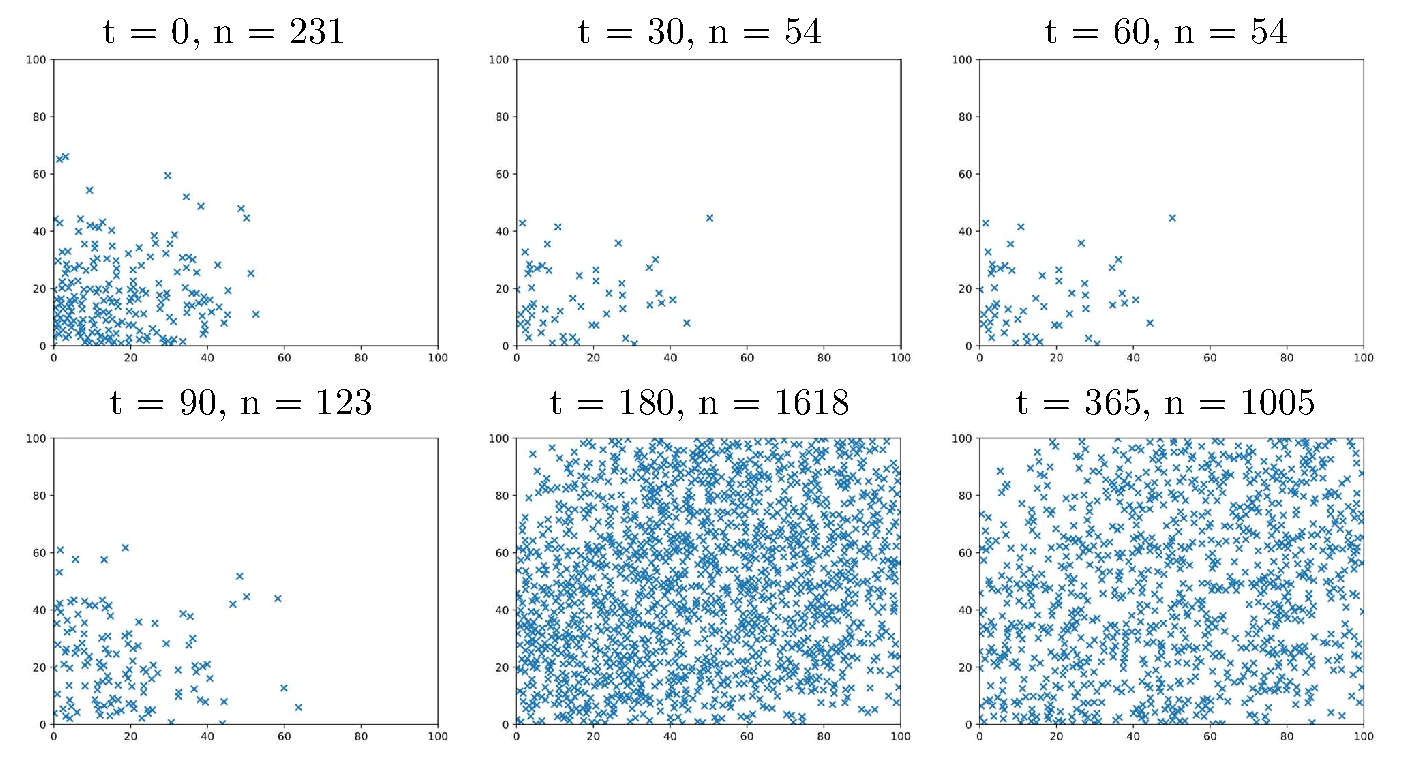
\includegraphics[scale=0.5]{figures/moderateclimatespread.pdf}
    \captionsetup{width=0.9\textwidth}
    \caption{\textbf{Dandelion spread over time in Clay, NY.} Each mark labels a spot where a dandelion (either in seed or plant phase) is located at that time stamp \(t\).}
    \label{fig:temperatespread}
\end{figure}

One exciting observation is that the stochastic seed dispersal process seems to cover the plot of land over time uniformly. However, it is essential to note that \textit{not all seeds survive} the dispersal process. After 30, 60, and 90 days of simulation from the beginning of the calendar year, the seeds began to travel even farther from the starting point. At the 180-day mark, we see an influx of seeds and dandelion plants due to the effects of optimal climate conditions for a dandelion's blooming phase. After the blooming phase, we see that through day 365, all surviving agents that are left are plants in their dormancy stage.

\begin{figure}[h!]
\centering
    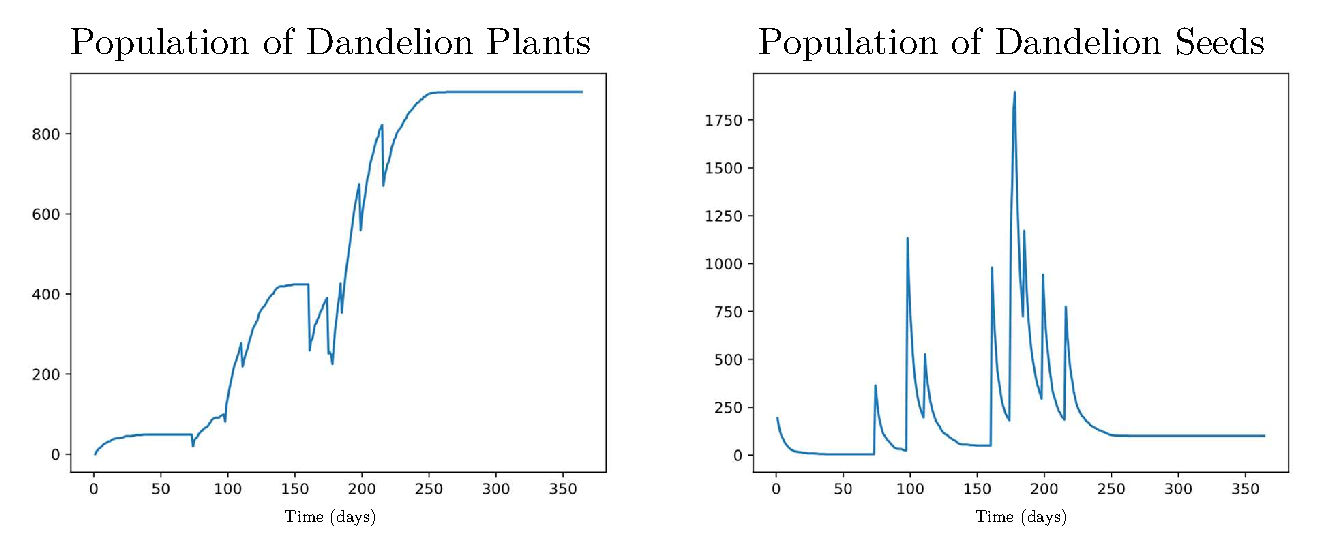
\includegraphics[scale=0.5]{figures/moderateclimatepopulation.pdf}
    \captionsetup{width=0.9\textwidth}
    \caption{\textbf{Growth in population of dandelion plants and seeds over time in Clay, NY.} The simulation began with a single puffball at coordinate \((0, 0)\).}
    \label{fig:temperatepopulation}
\end{figure}

A visualization of the growth (Figure~\ref{fig:temperatepopulation}) of the dandelion population and seed population over time shows us two key results:

\begin{enumerate}
    \item Dandelion plants go through two main blooming processes (spikes in population increase) throughout a year (spring and summer), which is consistent with other findings \cite{noauthor_dandelion_nodate-2}.
    \item Dandelion plant populations remain dormant in winter and fall months, while dandelion seeds do not spread much, or at all, in the colder months, which is a unique property of perennial plants \cite{noauthor_dandelion_nodate-2}.
\end{enumerate}

\subsubsection{Arid Region: Pheonix, AZ}

In Phoenix, Arizona, we obtained new climate and soil nutrition data from several sources \cite{arizona_guide_nodate, ottman_arizona_nodate, noauthor_average_nodate}. We then re-calibrated our model with these new hyperparameters and ran our simulated model.

\begin{figure}[h!]
\centering
    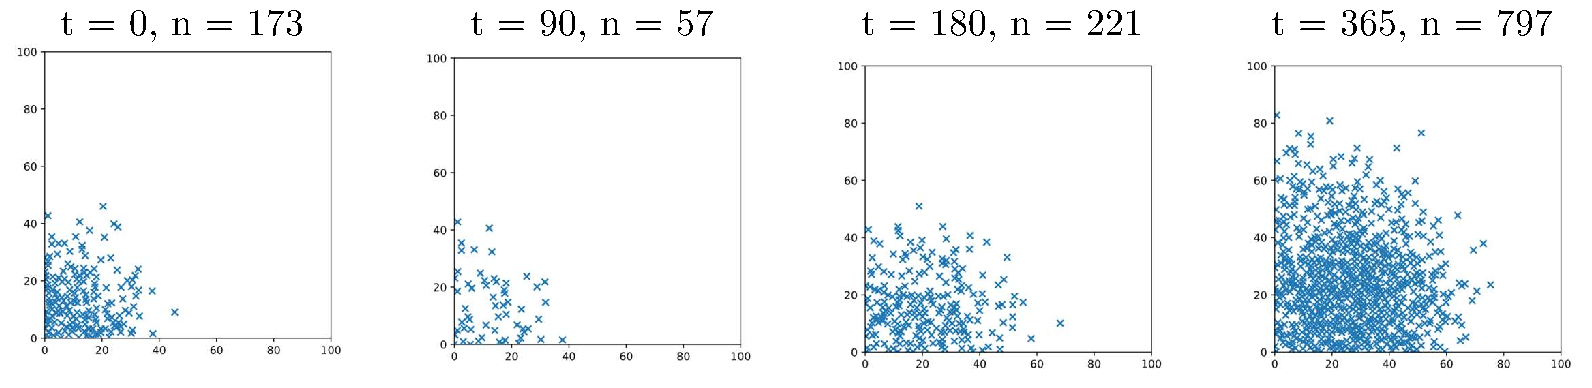
\includegraphics[scale=0.6]{figures/arizonaspread.pdf}
    \captionsetup{width=0.9\textwidth}
    \caption{\textbf{Dandelion spread over time in Phoenix, Arizona.}}
    \label{fig:arizonaspread}
\end{figure}

\begin{figure}[h!]
\centering
    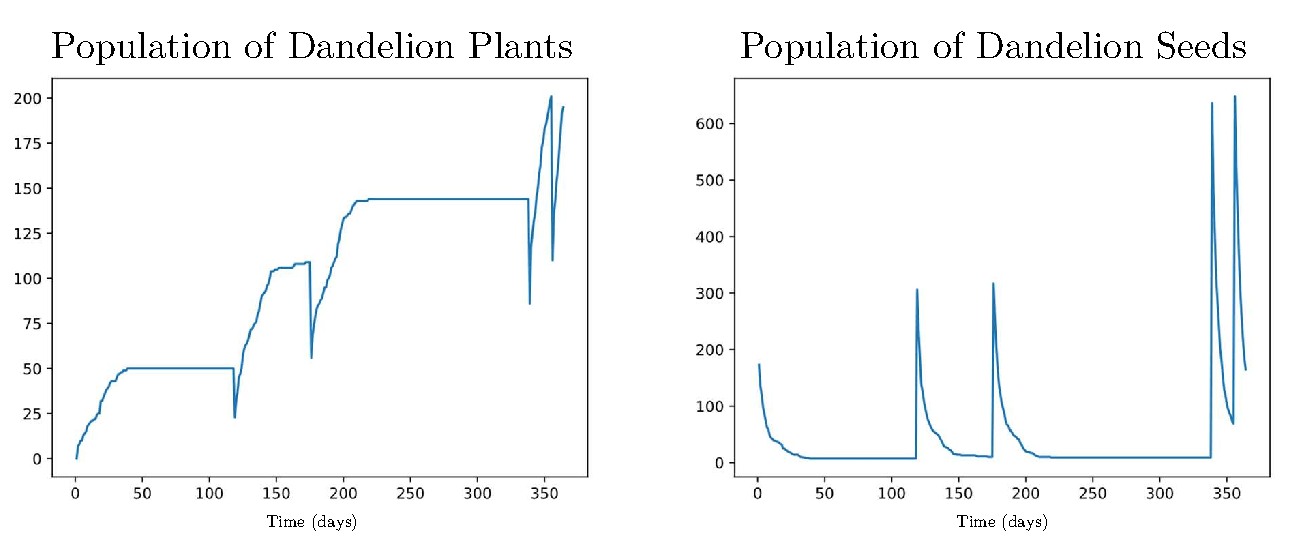
\includegraphics[scale=0.5]{figures/arizonapopulation.pdf}
    \captionsetup{width=0.9\textwidth}
    \caption{\textbf{Dandelion plant population growth in Phoenix, Arizona.}}
    \label{fig:arizonapopulation}
\end{figure}

One captivating observation of the spread of dandelions in an arid region is that their blooming seasons occur at different times of the year. This is most likely due to the availability of soil nutrients and optimal temperatures in the ending months of each year.

\subsubsection{Tropical Region: Florida Keys, FL}

By calibrating our model to Florida's tropical climate in the Florida Keys, we arrived at the following results for the dandelion growth and spread over one year. The calibrated climate data points were pulled from numerous sources as listed \cite{obreza_importance_2003, noauthor_average_nodate-1, pritchett_nitrogen_1959}.

One riveting observation of tropical regions is that blooming seasons tend to occur during winters at \(60-70^\circ\)F. Furthermore, we see that dandelion populations remain mostly stagnant over the summer months, as the summer heat may take away from dandelion growth. We can also conclude that dandelion populations follow a logistic growth pattern for the most part, which will be revisited in the following impact score model.

\begin{figure}[h!]
\centering
    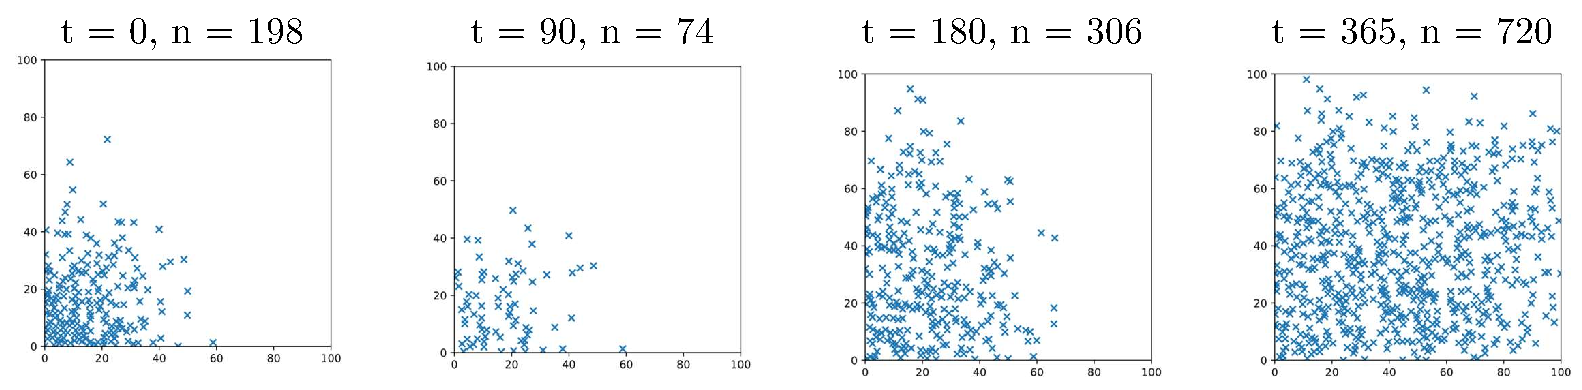
\includegraphics[scale=0.6]{figures/floridadistributions.pdf}
    \captionsetup{width=0.9\textwidth}
    \caption{\textbf{Dandelion spread over time in Florida Keys, Florida.} }
    \label{fig:floridaspread}
\end{figure}

\begin{figure}[h!]
\centering
    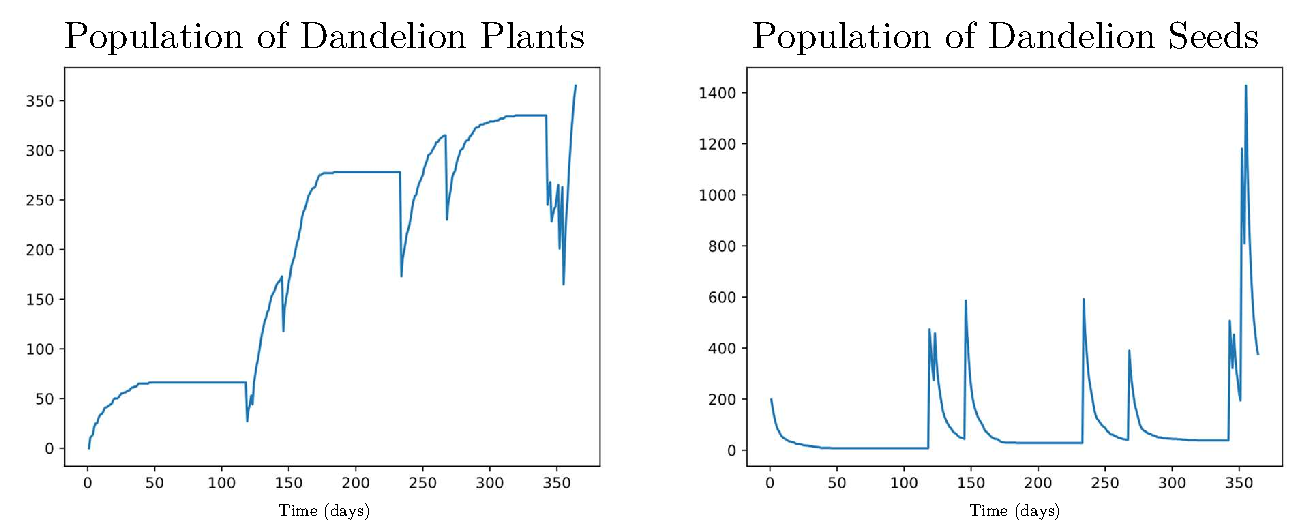
\includegraphics[scale=0.5]{figures/floridapopulation.pdf}
    \captionsetup{width=0.9\textwidth}
    \caption{\textbf{Dandelion plant population growth in Florida Keys, Florida.}}
    \label{fig:floridapopulation}
\end{figure}

